\documentclass[reqno,a4paper,12pt]{amsart}

\usepackage{amsmath,amssymb,amsthm,geometry,xcolor,soul,graphicx}
\usepackage{titlesec}
\usepackage{enumitem}
%\usepackage{enumerate}
\usepackage{lipsum}
\usepackage{listings}
\RequirePackage[most]{tcolorbox}
\usepackage{braket}
%\usepackage{esint} %$\varoiint$ (带圈的二重积分)
%\usepackage[colorlinks,linkcolor=red]{hyperref} %\url{}超链接
\usepackage{xeCJK}
\setCJKmainfont{Kai}
\geometry{left=0.7in, right=0.7in, top=1in, bottom=1in}

\renewcommand{\baselinestretch}{1.3}

\title{固体物理第七次作业}
\author{董建宇 ~~ 2019511017}

\begin{document}

\maketitle
\titleformat{\section}[hang]{\small}{\thesection}{0.8em}{}{}
\titleformat{\subsection}[hang]{\small}{\thesubsection}{0.8em}{}{}

\section{(12.3)\textbf{Crystal Structure} \\
The diagram of Fig. 12.22 shows a plan viem of a structure of cubic ZnS (zincblende) looking down the $z$ axis. The numbers attached to some atoms represent the heights of the atoms above the $z = 0$ plane expressed as a fraction of the cube edge $a$. UNlabeled atoms are $z = 0$ and $z = 0$. \\
(a) What is the Bravais lattice type? \\
(b) Describe the basis. \\
(c) Given that $a = 0.541nm$, calculate the nearest-neighbor Zn-Zn, Zn-S and S-S distances. \\
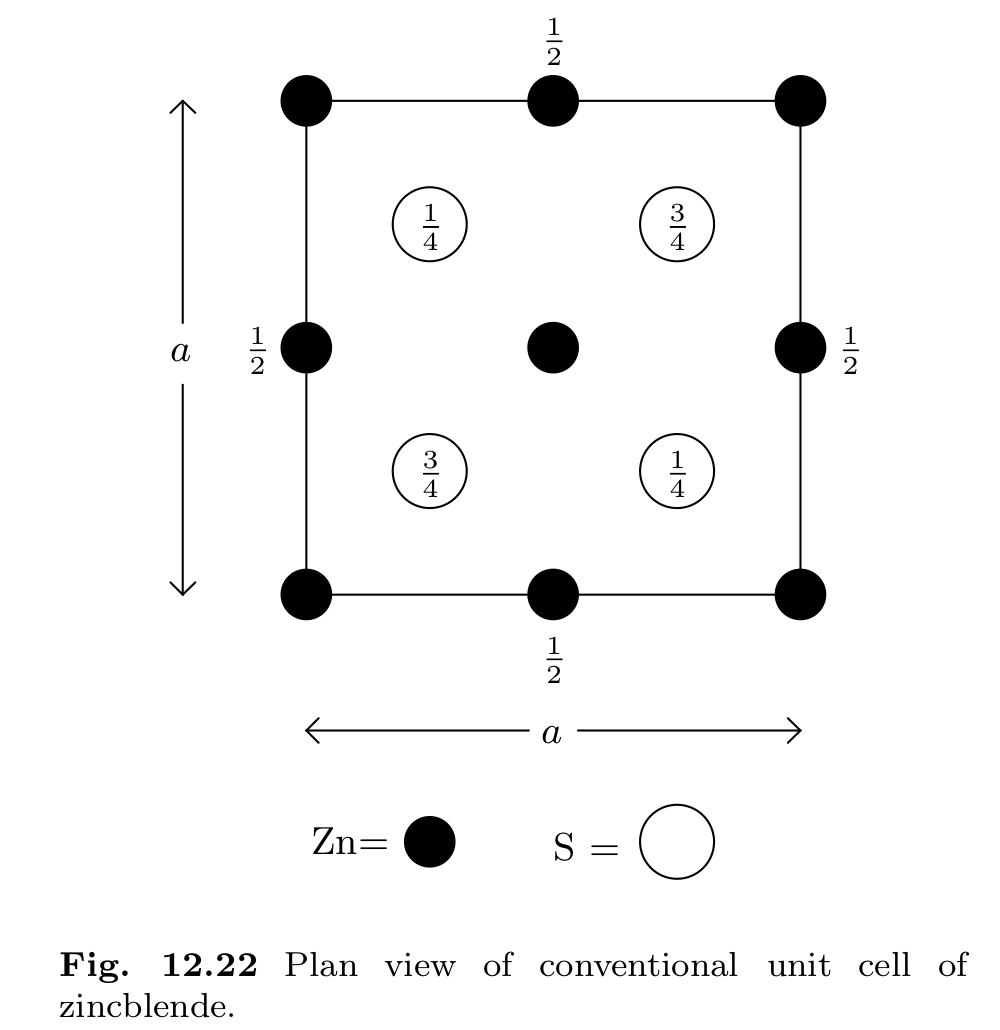
\includegraphics[scale = 0.19]{12.3.jpeg}}
\begin{tcolorbox}[breakable, colback = black!5!white, colframe = black]
晶体结构草图如下:(白色为S,其余为Zn)\\
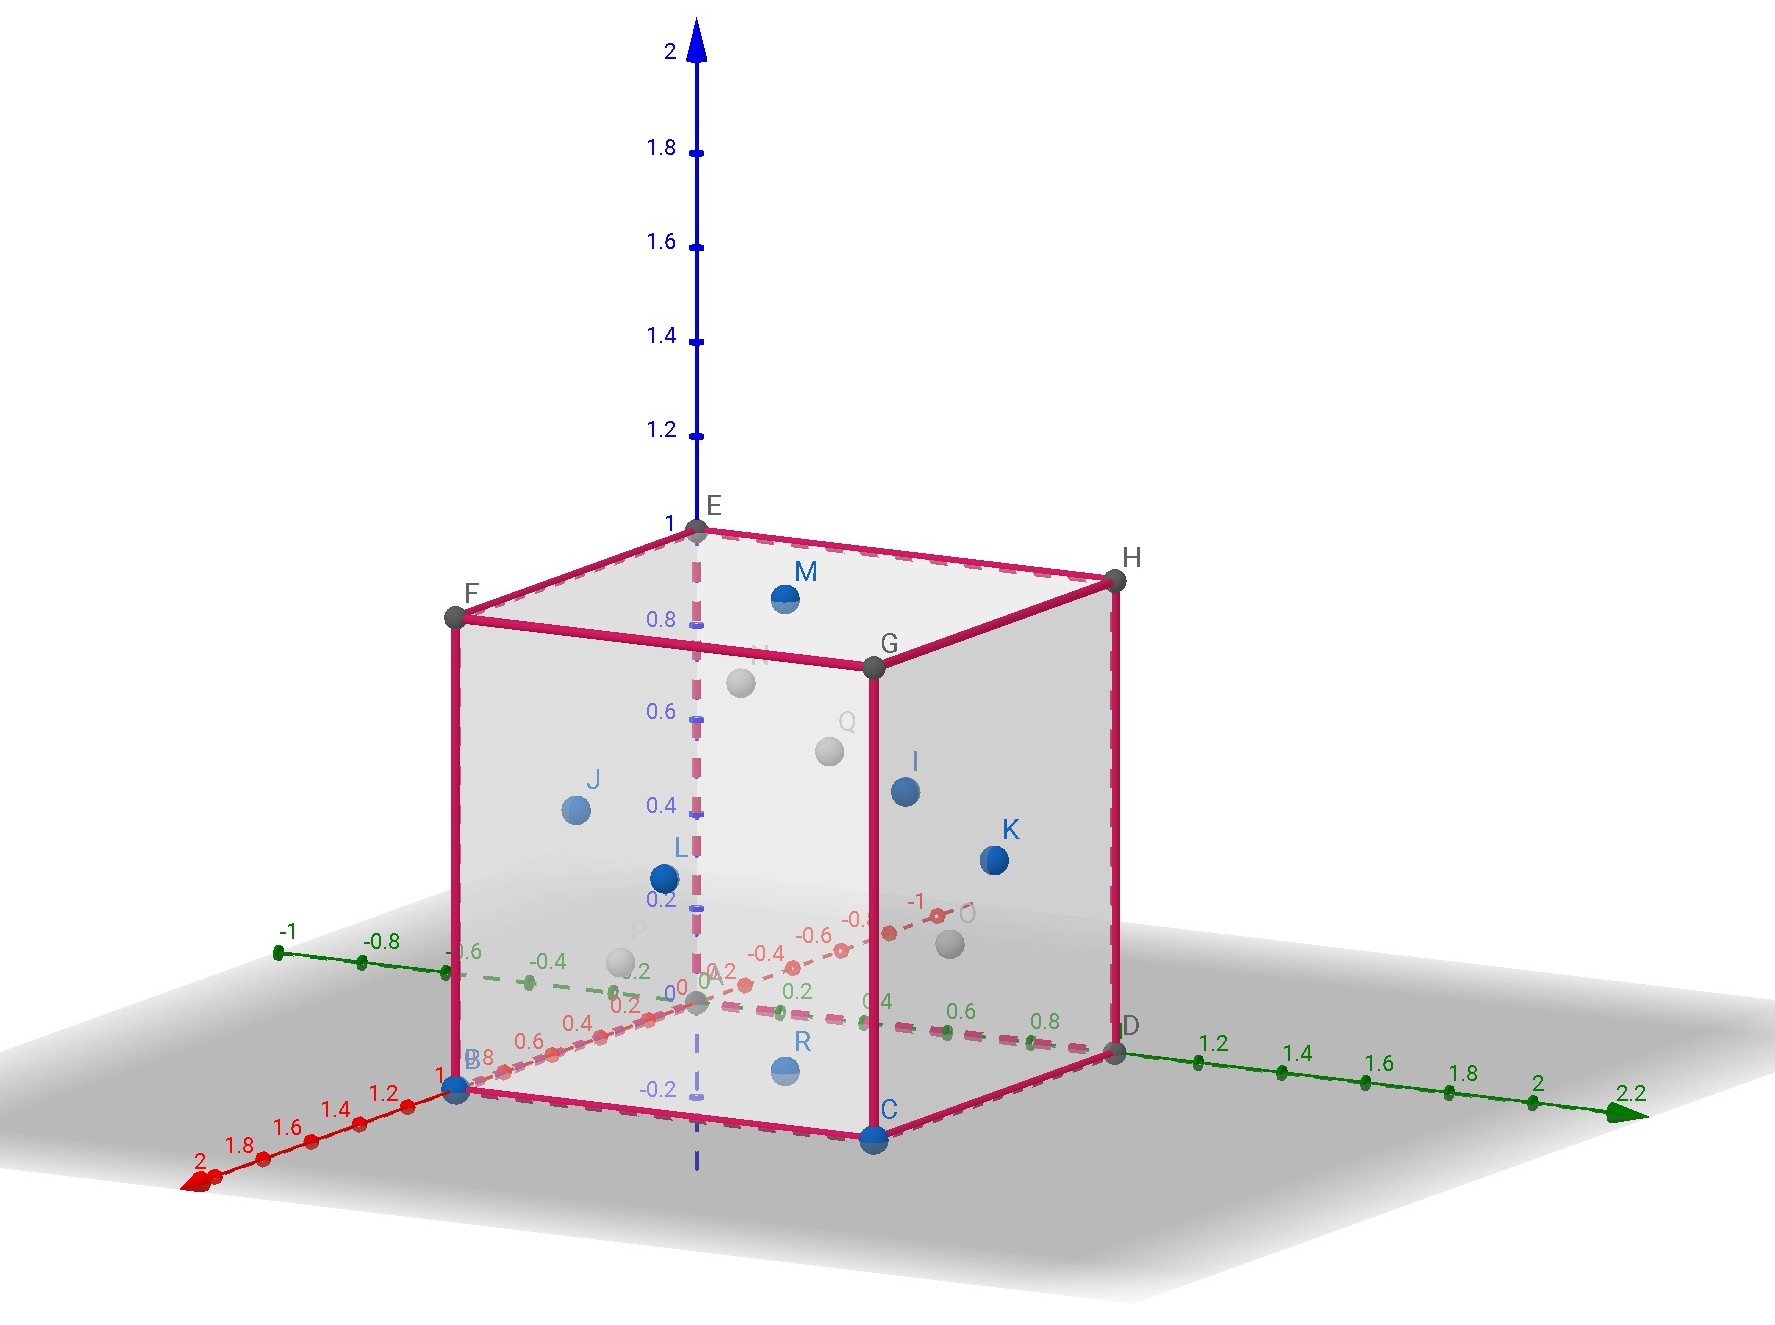
\includegraphics[scale = 0.16]{12.3structure.jpeg}
\begin{enumerate}[itemindent = -1.2em]
\item Bravais格子为面心立方结构(FCC)。 

\item 基为位于(0,0,0)的Zn原子与位于(0.25,0.25,0.75)的S原子。

\item 当$a = 0.541nm$时,最近邻Zn-Zn坐标分别为:(0,0,0)和(0,0.5,0.5),距离为:
\[
	d_1 = \frac{a}{\sqrt{2}} = 0.383nm.
\]
最近邻Zn-S坐标分别为:(0,0,1)和(0.25,0.25,0.75),距离为:
\[
	d_2 = a\sqrt{\frac{1}{16}\times 3} = 0.234nm.
\]
最近邻S-S坐标分别为:(0.25,0.25,0.75)和(0.75,0.75,0.75),距离为:
\[
	d_3 = \frac{a}{\sqrt{2}} = 0.383nm.
\]
\end{enumerate}
\end{tcolorbox}

\section{(12.4)\textbf{Packing Fractions} \\
Consider a lattice with a sphere at each lattice point. Choose the radius of the spheres to be such that neighboring spheres just touch (see fir example, Fig. 12.18). The packing fraction is the fraction of the volume of all of space which is enclosed by the union of all the spheres (i.e., the ratio of the volume of the spheres to the total volume). \\
(a) Calculate the packing fraction for a simple cubic lattice. \\
(b) Calculate the packing fraction for a bcc lattice. \\
(c) Calculate the packing fraction for a fcc lattice.}
\begin{tcolorbox}[breakable, colback = black!5!white, colframe = black]
\begin{enumerate}[itemindent = -1.5em]
\item 对于简单立方晶体,每个球的半径为$a/2$,其中$a$为立方晶格边长。则packing fraction 为:
\[
	\alpha_1 = \frac{\frac{4\pi}{3}\frac{a^3}{8}}{a^3} = \frac{\pi}{6}.
\]
\item 对于面心立方晶体,每个球的半径为:$\sqrt{3}a/4$。其中$a$为立方晶格边长。则packing fraction 为:
\[
	\alpha_2 = \frac{2\times \frac{4\pi}{3}\frac{3\sqrt{3}a^3}{64}}{a^3} = \frac{\sqrt{3}\pi}{8}.
\]
\item 对于体心立方晶体,每个球的半径为:$\sqrt{2}a/4$。其中$a$为立方晶格边长。则packing fraction 为:
\[
	\alpha_2 = \frac{4\times \frac{4\pi}{3}\frac{a^3}{16\sqrt{2}}}{a^3} = \frac{\pi}{3\sqrt{2}}.
\]
\end{enumerate}
\end{tcolorbox}

\section{(12.5)\textbf{Fluorine Beta Phase} \\
Fluorine can crystalize into a so-called beta-phase at temperatures between 45 and 55 Kelvin. Fig. 12.23 shows the cubic conventional unit cell for beta phase fluorine in three-dimensional form along with a plan view. \\
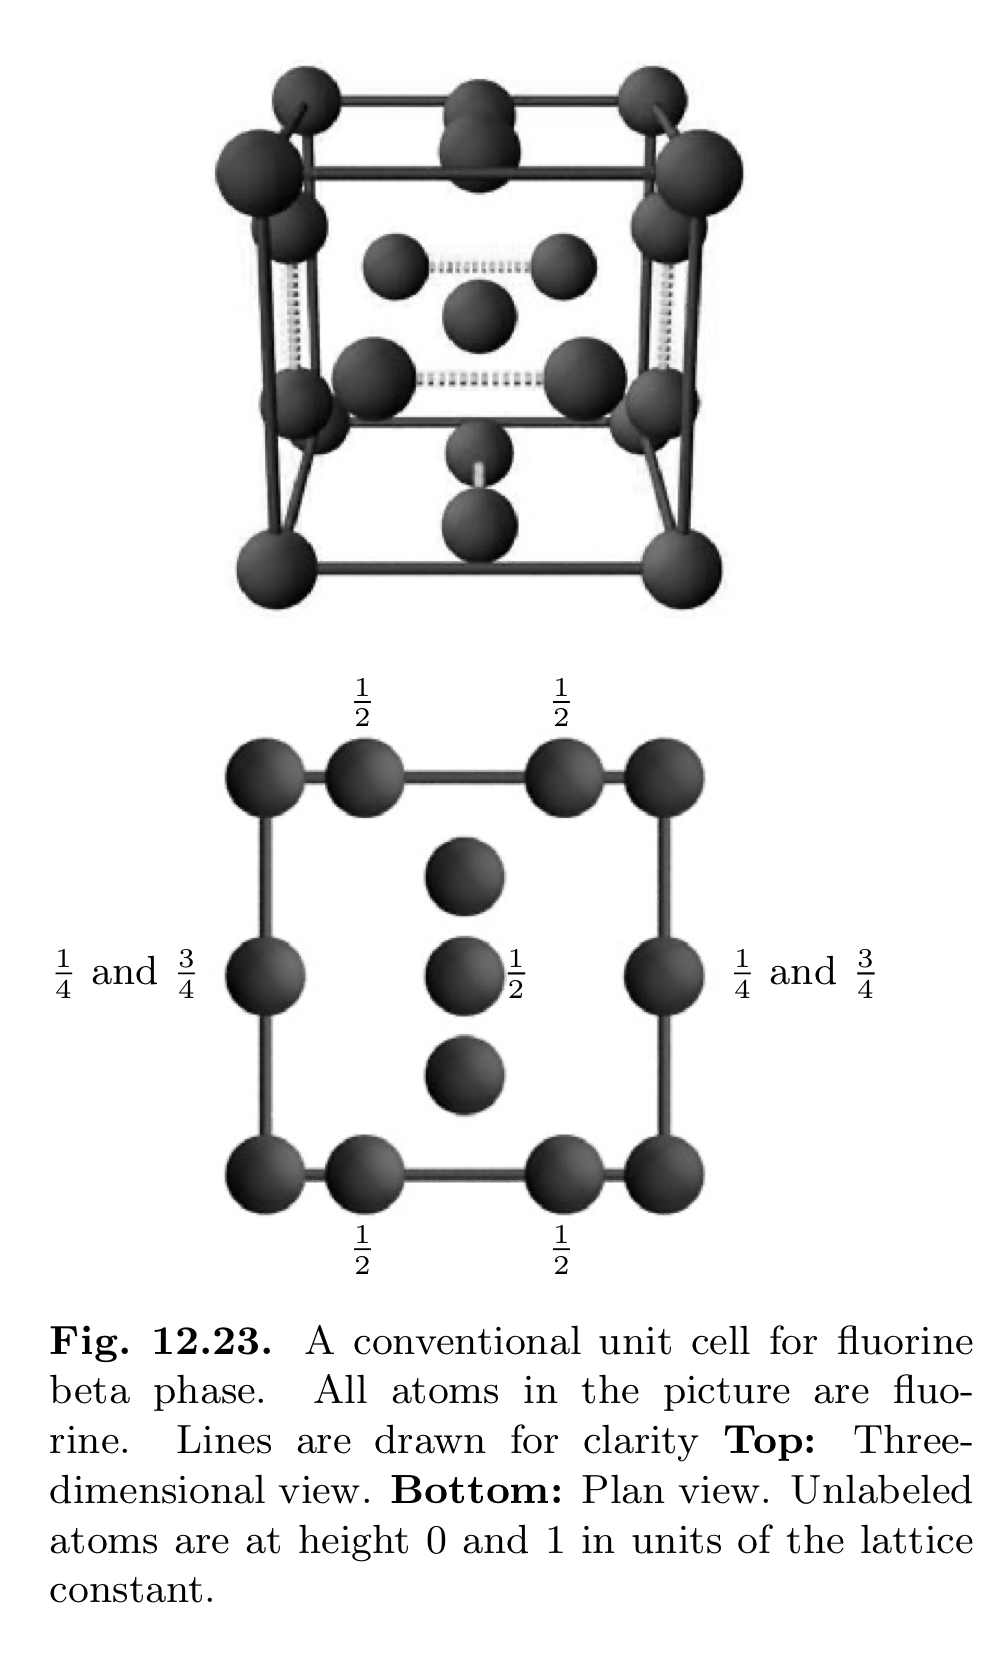
\includegraphics[scale = 0.19]{12.5.jpeg} \\
$\triangleright$ How many atoms are in this conventional unit cell? \\
$\triangleright$ What is the lattice and the basis for this crystal? }
\begin{tcolorbox}[breakable, colback = black!5!white, colframe = black]
注意到,8个顶点上的原子,每个有$\frac{1}{8}$处于元胞内,六个面上的原子,每个有$\frac{1}{2}$处于元胞内,还有元胞中心的原子,全部位于元胞内。则元胞内的总原子数为:
\[
	n = 8\times \frac{1}{8} + 12 \times \frac{1}{2} + 1 = 8.
\]
根据排除法可得:晶格为简单立方晶格(simple cubic)。 \\
基为传统元胞中相邻三个面内的原子,体心的原子以及一个顶点上的原子:(0,0,0); (0, 0.5, 0.25); (0, 0.5, 0.75); (0.5, 0.25,0); (0.5, 0.75, 0); (0.25, 0, 0.5); (0.75, 0, 0.5); (0.5, 0.5, 0.5)
\end{tcolorbox}

\end{document}